% Define markdown language for listings
\lstdefinelanguage{markdown}{
    basicstyle=\ttfamily,
    sensitive=false,
    breaklines=true,
    showstringspaces=false
}

% Define latex language for listings
\lstdefinelanguage{latex}{
    basicstyle=\ttfamily,
    sensitive=true,
    breaklines=true,
    showstringspaces=false
}

\chapter{Generative AI Usage}
Multiple generative AI tools were utilized as comprehensive assistants throughout this design project for three primary purposes: enhancing the linguistic quality and academic tone of technical documentation, converting data tables into properly formatted LaTeX code, and supporting the mockup design process through visual brainstorming and iteration. The primary tools used were Claude (Anthropic, version Sonnet 4.5) for text and code tasks, and Gemini (Google) and Nano Banana for visual mockup generation.

\section{Linguistic Enhancement}

\textbf{AI Tool Used:} Claude (Anthropic, Sonnet 4.5)

\textbf{Purpose:} Refining system architecture descriptions, improving the clarity and coherence of functional requirements, and ensuring consistent academic tone throughout the design document while maintaining technical precision.

\textbf{Typical Usage Pattern:} Initial drafts containing technical concepts and design decisions were written by the authors and subsequently submitted to the AI with prompts requesting linguistic refinement and academic style optimization. The AI provided alternative phrasings, improved sentence structure, and enhanced readability.

\textbf{Example Prompt:}
\begin{verbatim}
"Rewrite the following text in proper academic English, 
maintaining technical accuracy and improving clarity"
\end{verbatim}

\textbf{Before:} "This chapter provides visual representations of the mobile application user interface for all main user flows, illustrating the design and functionality of the system. Each mockup refers to what was previously described in the UI section of the RASD document related to the BBP platform. Each section describes a specific flow, going from left to right and passing then to other rows. User experience was a core aspect kept in mind while designing these interfaces and users interactions"

\textbf{After:} "This chapter presents visual representations of the mobile application's user interface, covering all main user flows. Each mockup corresponds to the UI specifications previously described in the RASD document for the BBP platform. The sections are organized by flow, with screens arranged from left to right and continuing across rows. User experience was a central consideration throughout the design of these interfaces and interactions."

\textbf{Human Verification:} All AI-generated linguistic improvements were carefully reviewed, edited where necessary, and validated by the authors to ensure technical accuracy and consistency with the BBP system design specifications.

\section{LaTeX Table Generation}

\textbf{AI Tool Used:} Claude (Anthropic, Sonnet 4.5)

\textbf{Purpose:} Converting data tables from Google Sheets and Excel spreadsheets into properly formatted LaTeX code, ensuring consistent styling, appropriate column widths, and professional presentation suitable for academic documentation.

\textbf{Typical Usage Pattern:} Tabular data prepared in spreadsheet applications was exported as CSV and provided to the AI along with specific formatting requirements (e.g., column alignment, caption text, label references). The AI generated complete LaTeX table code ready for integration into the document.

\textbf{Example Prompt:}
\begin{lstlisting}[language=markdown]
"Convert this Excel table, exported as CSV, into LaTeX format.
\end{lstlisting}

\textbf{Input Data (from Excel/Google Sheets):}
\begin{lstlisting}[language=markdown]
Req ID;Description (Summary);Mapped Design Components
R1;Allow unregistered User to sign up;Auth Service, API Gateway, Mobile App, Auth DB
R2;Allow registered Users to login;Auth Service, API Gateway, Mobile App, Auth DB
R3;Manually insert a bike path (streets/status);Trip Service, Mobile App, API Gateway, Map Service Adapter

continue...
\end{lstlisting}

\textbf{Generated LaTeX Code:}
\lstset{
    language=latex
}
\begin{lstlisting}[language=latex]
\begin{tabular}{|l|p{6cm}|p{7cm}|}
\hline
\textbf{Req ID} & \textbf{Description (Summary)} & \textbf{Mapped Design Components} \\
\hline
R1 & Allow unregistered User to sign up & Mobile App, API Gateway, Auth Service, Auth DB \\
\hline
R2 & Allow registered Users to login & Mobile App, API Gateway, Auth Service, Auth DB \\
\hline
R3 & Manually insert a bike path (streets/status) & Mobile App, API Gateway, Trip Service, Map Service Adapter \\
\hline

continue...
\end{lstlisting}

\textbf{Human Verification:} All generated LaTeX tables were compiled and visually inspected to ensure correct rendering. Data accuracy was verified against source spreadsheets, and formatting was adjusted where necessary to maintain document-wide consistency.

\section{Mockup Design Brainstorming}

\textbf{AI Tools Used:} Gemini (Google) and Nano Banana for image generation;

\textbf{Purpose:} Supporting the iterative mockup design process by generating visual concepts from hand-drawn wireframes, providing design inspiration for final mockups creations.

\textbf{Design Process:}

\subsection{Phase 1: Wireframe Creation}
Hand-drawn wireframes were created to establish basic layout structure, component placement, and information hierarchy. These wireframes captured essential functional elements and user interactions.

\subsection{Phase 2: AI-Generated Mockup Concepts}
The hand-drawn wireframes were provided to the AI with detailed prompts describing the desired visual style, color scheme, and design aesthetic.

Provided prompt also included \href{https://claude.com/blog/improving-frontend-design-through-skills}{frontend-design skill} from Anthropic which aims to reduce AI slop in mockup designing.

\textbf{Example Prompt:}
\begin{lstlisting}[language=markdown]
"Given the following wireframes of Best Bike Paths system, for each screen create a mockup.

This app aims to provide both automatically and manually recording of bike trips you perform. Additionally there's a community list of path managed by system as aggregation of multiple trips performed by different users. It involves accelerometer, gyroscope analysis for detecting potholes. Users can see their past histories of trips, keeps them private or publish them to contribute to community path management. It uses weather for past conditions and currents condition along currently visualizing trajectories on map

Use #83E084 #DCE0CA #E0DD84 as base colors

iOS app, light moded, figma style, 9:19 aspect ratio, no phone frame

-----
<FRONTEND_DESIGN_SKILL_PROMPT>

\end{lstlisting}

\textbf{AI-Generated Outputs:}
The AI image generation tools (Gemini and Nano Banana) generated mockups images.

\subsection{Phase 3: Final Mockup Development}
The AI-generated mockups served as visual inspiration and design exploration. We then created final mockups using professional design tools (Figma), incorporating successful elements from the AI-generated concepts while maintaining consistency with established design systems and accessibility standards.

\textbf{Design Timeline Visualization:}

\begin{figure}[H]
\centering
\begin{subfigure}{\textwidth}
    \centering
    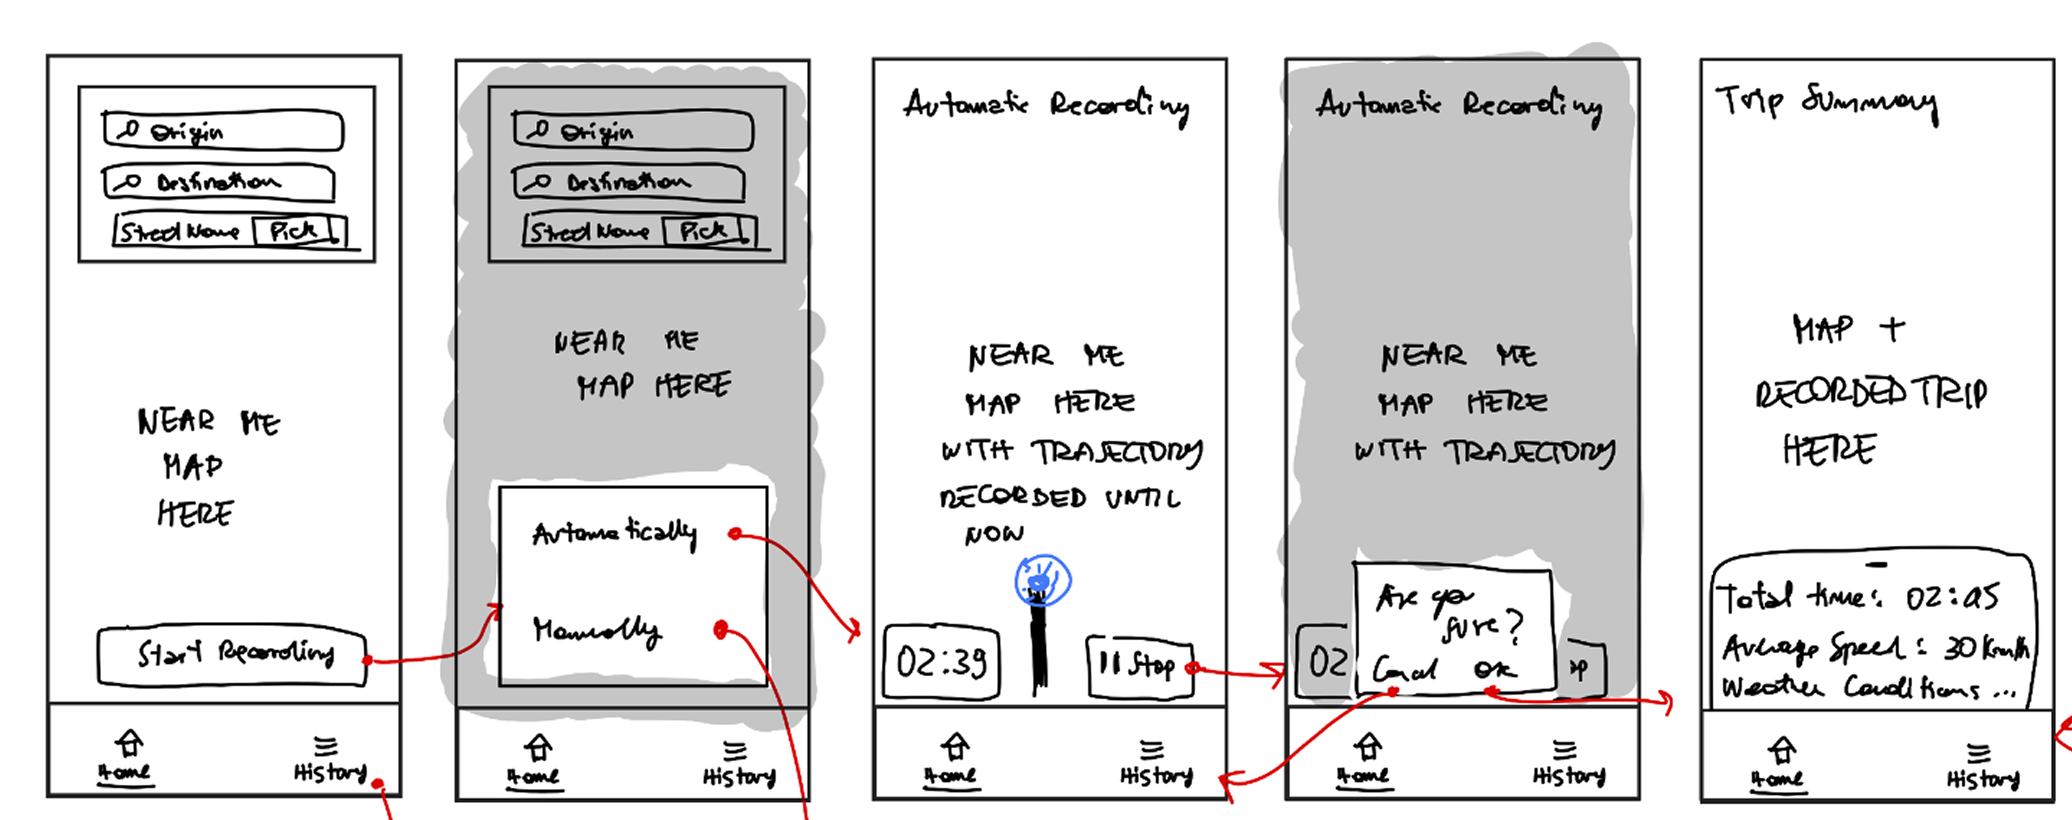
\includegraphics[width=0.6\textwidth]{DD/images/wireframe.png}
    \caption{Hand-drawn wireframe}
    \label{fig:wireframe}
\end{subfigure}

\vspace{0.5cm}

\begin{subfigure}{\textwidth}
    \centering
    \includegraphics[width=0.6\textwidth]{DD/images/mockup_inspiration.png}
    \caption{AI-generated concept}
    \label{fig:mockup_concept}
\end{subfigure}

\vspace{0.5cm}

\begin{subfigure}{\textwidth}
    \centering
    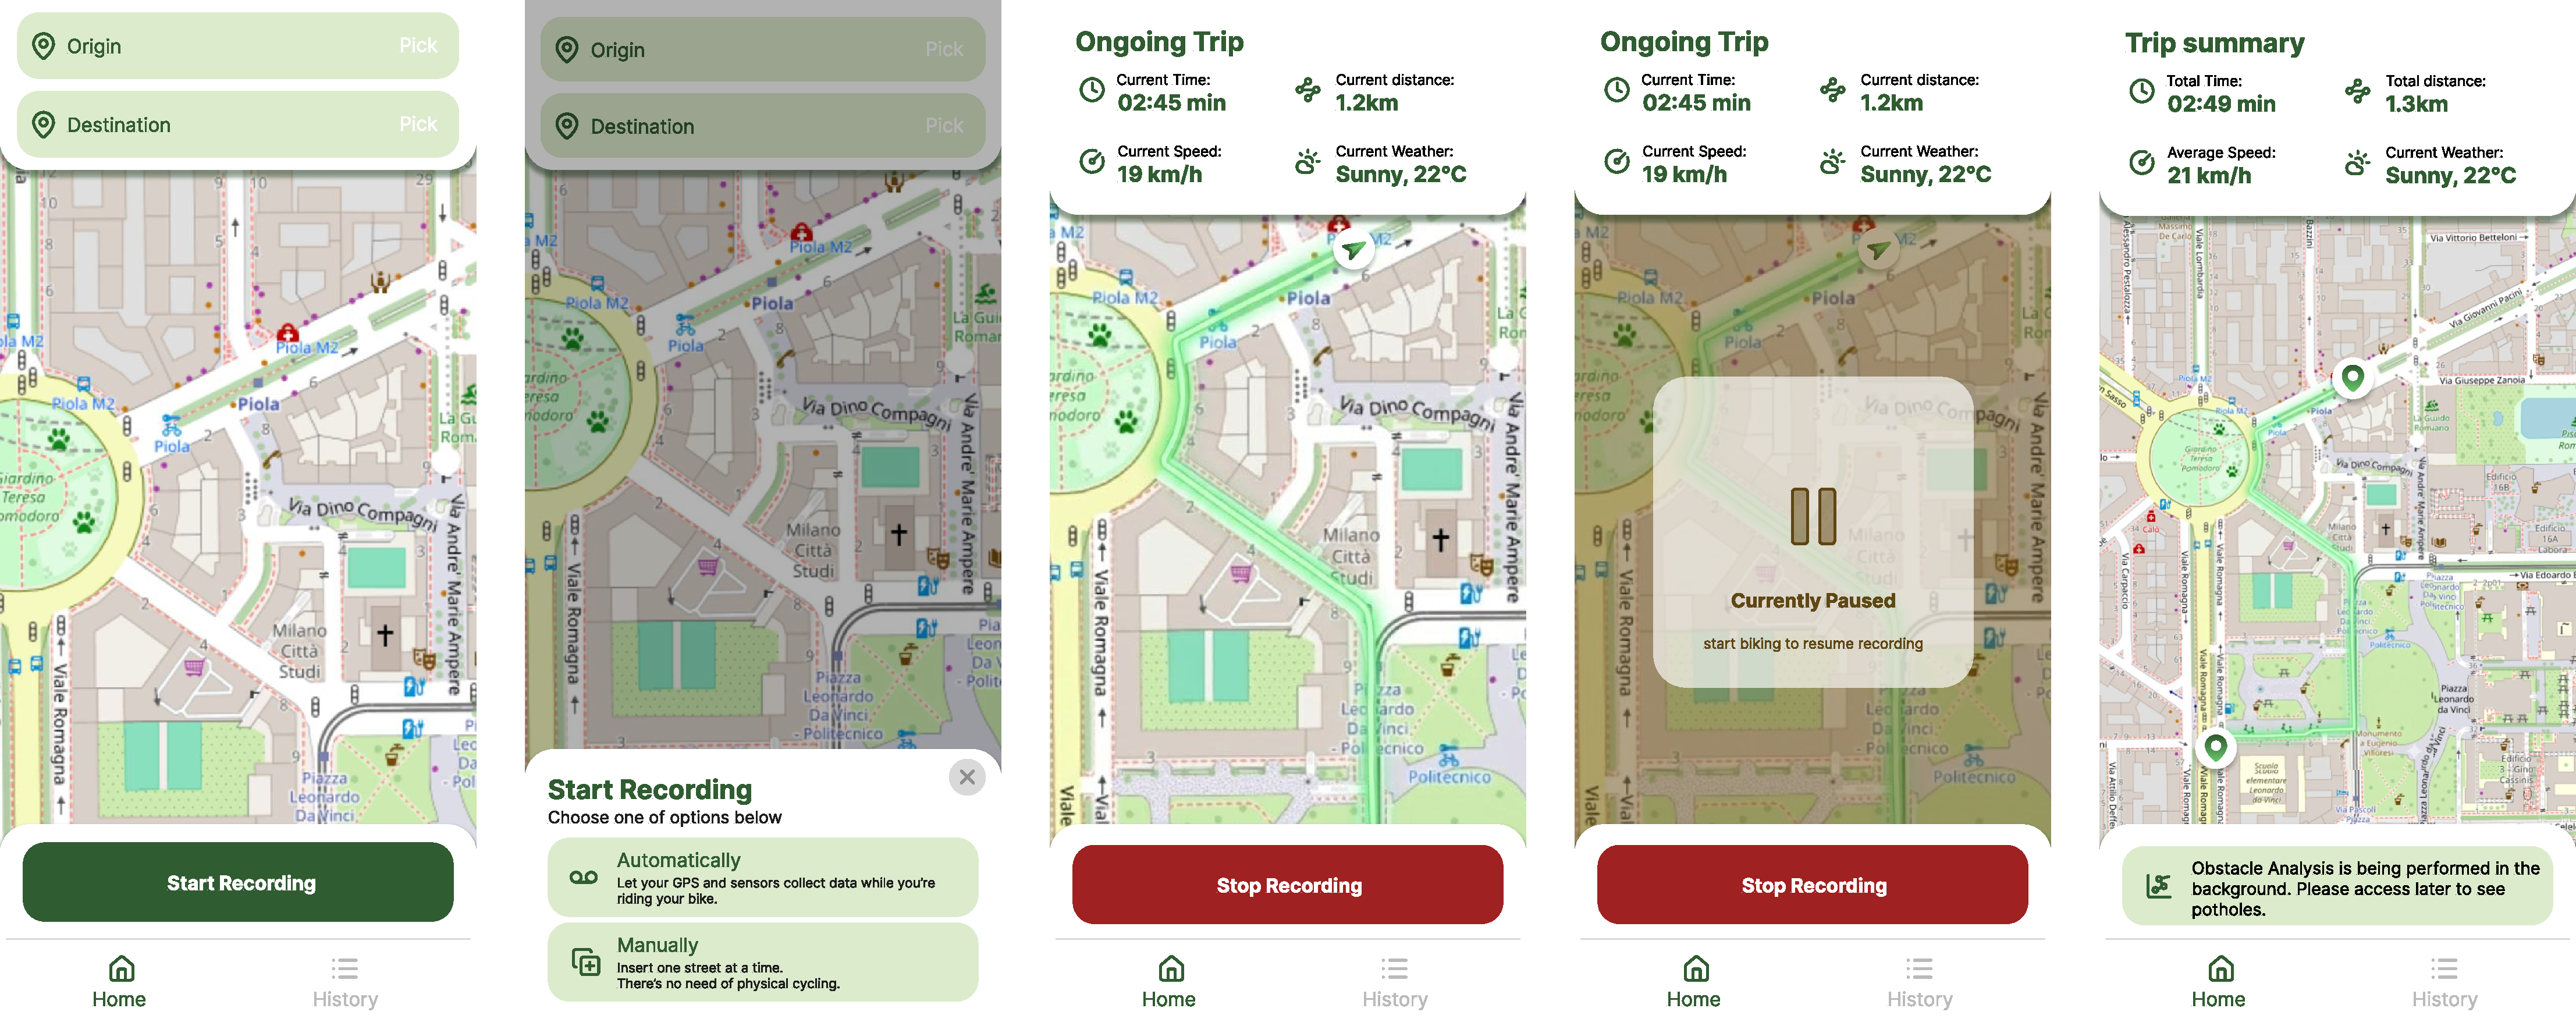
\includegraphics[width=0.6\textwidth]{DD/images/mockups/AUTOMATIC_RECORDING_FLOW.pdf}
    \caption{Final professional mockup}
    \label{fig:mockup_final}
\end{subfigure}

\caption{Mockup design evolution: from initial wireframe through AI-assisted brainstorming to final implementation}
\label{fig:mockup_evolution}
\end{figure}

\textbf{Human Control and Verification:}
All final mockups were created by human designers using professional design tools. AI-generated images served solely as inspiration and were not directly incorporated into the final deliverables. Design decisions regarding layout, accessibility, visual consistency and user experience remained under complete human control.

\vspace{1em}
\noindent\textit{Note:} All substantive design decisions, system architecture, functional specifications, and final visual designs remain the original work of the author(s). AI assistance was limited to linguistic refinement, LaTeX code generation, and preliminary design exploration only. All technical content and design deliverables were created, reviewed, and validated by the project team.